\documentclass[12pt, a4paper]{article}
\usepackage[utf8]{inputenc}
\usepackage{geometry}
\usepackage{graphicx}
\usepackage{tikz}
\usepackage{tabularx}
\usepackage{multicol}
\usepackage{multirow}
\usepackage{array,booktabs,ragged2e}
\usepackage{amsmath}
\usepackage{xkeyval}
\usepackage{float}
\usepackage{physics}
\usepackage{tfrupee}
\usepackage{mathtools} %underbrace symbol
\usepackage{adjustbox} 
\usepackage{xcolor}
\usepackage{colortbl}
\usepackage{tkz-euclide}
\usepackage{pgf-pie}
\usepackage[misc]{ifsym} %Used in tally mark
\usetikzlibrary{patterns,calc}

\newcommand{\scalefactor}{1}


\geometry{top=2.5cm, bottom=1.25cm, left=1.5cm, right=1.5cm}
\makeatletter
%-----------------------------------------------------------
% text bottom 4 option in 1 row
%-----------------------------------------------------------

\define@key{mcqtextbottomFourOne}{questionnumber}{\def\mcqtextbottomFourOnequestionnumber{#1}} 
\define@key{mcqtextbottomFourOne}{questionTag}{\def\mcqtextbottomFourOnequestionTag{#1}}
\define@key{mcqtextbottomFourOne}{questiontext}{\def\mcqtextbottomFourOnequestiontext{#1}}
\define@key{mcqtextbottomFourOne}{optionA}{\def\mcqtextbottomFourOneoptionA{#1}}
\define@key{mcqtextbottomFourOne}{optionB}{\def\mcqtextbottomFourOneoptionB{#1}}
\define@key{mcqtextbottomFourOne}{optionC}{\def\mcqtextbottomFourOneoptionC{#1}}
\define@key{mcqtextbottomFourOne}{optionD}{\def\mcqtextbottomFourOneoptionD{#1}}
\define@key{mcqtextbottomFourOne}{correctoption}{\def\mcqtextbottomFourOnecorrectoption{#1}}


\newcommand{\mcqtextbottomFourOne}[1]{%
\setkeys{mcqtextbottomFourOne}{#1}%
\vspace{2.5mm}
\begin{raggedright}
\textbf{Question Tag:} \mcqtextbottomFourOnequestionTag \hfill \textbf{Correct Option:} \mcqtextbottomFourOnecorrectoption\\
\end{raggedright}
\vspace{\baselineskip}
\begin{raggedright}
\textbf{Question \mcqtextbottomFourOnequestionnumber:} \mcqtextbottomFourOnequestiontext\\
\medskip
(a) \medskip \mcqtextbottomFourOneoptionA\\
(b) \medskip \mcqtextbottomFourOneoptionB\\      
(c) \medskip \mcqtextbottomFourOneoptionC\\
(d) \medskip \mcqtextbottomFourOneoptionD\\
\end{raggedright}
}

%-----------------------------------------------------------

%-----------------------------------------------------------

% DEFINE KEY FOR mcqtextbottomOneFour %

\define@key{mcqtextbottomOneFour}{questionnumber}{\def\mcqtextbottomOneFourquestionnumber{#1}} 
\define@key{mcqtextbottomOneFour}{questiontext}{\def\mcqtextbottomOneFourquestiontext{#1}}
\define@key{mcqtextbottomOneFour}{optionA}{\def\mcqtextbottomOneFouroptionA{#1}}
\define@key{mcqtextbottomOneFour}{optionB}{\def\mcqtextbottomOneFouroptionB{#1}}
\define@key{mcqtextbottomOneFour}{optionC}{\def\mcqtextbottomOneFouroptionC{#1}}
\define@key{mcqtextbottomOneFour}{optionD}{\def\mcqtextbottomOneFouroptionD{#1}}
\define@key{mcqtextbottomOneFour}{questionTag}{\def\mcqtextbottomOneFourquestionTag{#1}} 
\define@key{mcqtextbottomOneFour}{correctoption}{\def\mcqtextbottomOneFourcorrectoption{#1}}

% COMMAND FOR mcqtextbottomOneFour %

\newcommand{\mcqtextbottomOneFour}[1]{%
\setkeys{mcqtextbottomOneFour}{#1}%
\vspace{2.5mm}
\begin{raggedright}
\textbf{Question Tag:} \mcqtextbottomOneFourquestionTag \hfill \textbf{Correct Option:} \mcqtextbottomOneFourcorrectoption\\
\end{raggedright}
\vspace{\baselineskip}
\begin{raggedright}
\textbf{Question \mcqtextbottomOneFourquestionnumber:} \mcqtextbottomOneFourquestiontext
\begin{multicols}{4}
(a) \medskip \mcqtextbottomOneFouroptionA\\
(b) \medskip \mcqtextbottomOneFouroptionB\\      
(c) \medskip \mcqtextbottomOneFouroptionC\\
(d) \medskip \mcqtextbottomOneFouroptionD\\
\end{multicols}
\end{raggedright}
}

%-----------------------------------------------------------

%-----------------------------------------------------------

% Define key FOR mcqtextbottomOneTwo 

\define@key{mcqtextbottomOneTwo}{questionnumber}{\def\mcqtextbottomOneTwoquestion{#1}}
\define@key{mcqtextbottomOneTwo}{questiontext}{\def\mcqtextbottomOneTwoquestiontext{#1}}
\define@key{mcqtextbottomOneTwo}{optionA}{\def\mcqtextbottomOneTwooptionA{#1}}
\define@key{mcqtextbottomOneTwo}{optionB}{\def\mcqtextbottomOneTwooptionB{#1}}
\define@key{mcqtextbottomOneTwo}{questionTag}{\def\mcqtextbottomOneTwoquestionTag{#1}}
\define@key{mcqtextbottomOneTwo}{correctoption}{\def\mcqtextbottomOneTwocorrectoption{#1}}

% COMMAND FOR mcqtextbottomOneTwo %

\newcommand{\mcqtextbottomOneTwo}[1]{%
\setkeys{mcqtextbottomOneTwo}{#1}%
\vspace{2.5mm}
\begin{raggedright}
\textbf{Question Tag:} \mcqtextbottomOneTwoquestionTag \hfill \textbf{Correct Option:} \mcqtextbottomOneTwocorrectoption\\
\end{raggedright}
\vspace{\baselineskip}
\begin{raggedright}
\textbf{Question \mcqtextbottomOneTwoquestion:} \mcqtextbottomOneTwoquestiontext\\
\begin{multicols}{2}
(a) \medskip \mcqtextbottomOneTwooptionA\\
(b) \medskip \mcqtextbottomOneTwooptionB\\
\end{multicols}
\end{raggedright}
}

%-----------------------------------------------------------

%-----------------------------------------------------------

% Define key FOR mcqtextbottomTwoTwo

\define@key{mcqtextbottomTwoTwo}{questionnumber}{\def\mcqtextbottomTwoTwoquestion{#1}}
\define@key{mcqtextbottomTwoTwo}{questiontext}{\def\mcqtextbottomTwoTwoquestiontext{#1}}
\define@key{mcqtextbottomTwoTwo}{optionA}{\def\mcqtextbottomTwoTwooptionA{#1}}
\define@key{mcqtextbottomTwoTwo}{optionB}{\def\mcqtextbottomTwoTwooptionB{#1}}
\define@key{mcqtextbottomTwoTwo}{optionC}{\def\mcqtextbottomTwoTwooptionC{#1}}
\define@key{mcqtextbottomTwoTwo}{optionD}{\def\mcqtextbottomTwoTwooptionD{#1}}
\define@key{mcqtextbottomTwoTwo}{questionTag}{\def\mcqtextbottomTwoTwoquestionTag{#1}}
\define@key{mcqtextbottomTwoTwo}{correctoption}{\def\mcqtextbottomTwoTwocorrectoption{#1}}

% COMMAND FOR mcqtextbottomTwoTwo %

\newcommand{\mcqtextbottomTwoTwo}[1]{%
\setkeys{mcqtextbottomTwoTwo}{#1}%
\vspace{1.5mm}
\begin{raggedright}
\textbf{Question Tag:} \mcqtextbottomTwoTwoquestionTag \hfill \textbf{Correct Option:} \mcqtextbottomTwoTwocorrectoption\\
\end{raggedright}
\vspace{\baselineskip}
\begin{raggedright}
\textbf{Question \mcqtextbottomTwoTwoquestion:} \mcqtextbottomTwoTwoquestiontext\\
\begin{multicols}{2}
(a) \medskip \mcqtextbottomTwoTwooptionA\\
(c) \medskip \mcqtextbottomTwoTwooptionC\\
\columnbreak
(b) \medskip \mcqtextbottomTwoTwooptionB\\
(d) \medskip \mcqtextbottomTwoTwooptionD\\
\end{multicols}
\end{raggedright}
\vspace{5mm}
}

%-----------------------------------------------------------

%-----------------------------------------------------------

% Define key FOR mcqtextsideFourOne


\define@key{mcqtextsideFourOne}{questionnumber}{\def\mcqtextsideFourOnequestionnumber{#1}} 
\define@key{mcqtextsideFourOne}{questionTag}{\def\mcqtextsideFourOnequestionTag{#1}} 
\define@key{mcqtextsideFourOne}{questiontext}{\def\mcqtextsideFourOnequestiontext{#1}}
\define@key{mcqtextsideFourOne}{optionA}{\def\mcqtextsideFourOneoptionA{#1}}
\define@key{mcqtextsideFourOne}{optionB}{\def\mcqtextsideFourOneoptionB{#1}}
\define@key{mcqtextsideFourOne}{optionC}{\def\mcqtextsideFourOneoptionC{#1}}
\define@key{mcqtextsideFourOne}{optionD}{\def\mcqtextsideFourOneoptionD{#1}}
\define@key{mcqtextsideFourOne}{correctoption}{\def\mcqtextsideFourOnecorrectoption{#1}}
\define@key{mcqtextsideFourOne}{leftmini}{\def\mcqtextsideFourOneleftmini{#1}}
\define@key{mcqtextsideFourOne}{rightmini}{\def\mcqtextsideFourOnerightmini{#1}}

% COMMAND FOR mcqtextsideFourOne

\newcommand{\mcqtextsideFourOne}[1]{%
\setkeys{mcqtextsideFourOne}{#1}%
\vspace{2.5mm}
\begin{raggedright}
\textbf{Question Tag:} \mcqtextsideFourOnequestionTag \hfill \textbf{Correct Option:} \mcqtextsideFourOnecorrectoption\\
\end{raggedright}
\vspace{\baselineskip}
\begin{raggedright}
\begin{minipage}[t]{\mcqtextsideFourOneleftmini\linewidth}
\textbf{Question \mcqtextsideFourOnequestionnumber:} \mcqtextsideFourOnequestiontext\\
\end{minipage}\hfill
\begin{minipage}[t]{\mcqtextsideFourOnerightmini\linewidth}
(a) \medskip \mcqtextsideFourOneoptionA\\
(b) \medskip \mcqtextsideFourOneoptionB\\
(c) \medskip \mcqtextsideFourOneoptionC\\
(d) \medskip \mcqtextsideFourOneoptionD\\
\end{minipage}
\end{raggedright}
}

%-----------------------------------------------------------

%-----------------------------------------------------------

% Define key FOR mcqimgbottomOneFour

\define@key{mcqimgbottomOneFour}{questionnumber}{\def\mcqimgbottomOneFourquestionnumber{#1}}
\define@key{mcqimgbottomOneFour}{questionTag}{\def\mcqimgbottomOneFourquestionTag{#1}}
\define@key{mcqimgbottomOneFour}{questiontext}{\def\mcqimgbottomOneFourquestiontext{#1}}
\define@key{mcqimgbottomOneFour}{optionA}{\def\mcqimgbottomOneFouroptionA{#1}}
\define@key{mcqimgbottomOneFour}{optionB}{\def\mcqimgbottomOneFouroptionB{#1}}
\define@key{mcqimgbottomOneFour}{optionC}{\def\mcqimgbottomOneFouroptionC{#1}}
\define@key{mcqimgbottomOneFour}{optionD}{\def\mcqimgbottomOneFouroptionD{#1}}
\define@key{mcqimgbottomOneFour}{correctoption}{\def\mcqimgbottomOneFourcorrectoption{#1}}

% COMMAND FOR mcqimgbottomOneFour %

\newcommand{\mcqimgbottomOneFour}[1]{%
\setkeys{mcqimgbottomOneFour}{#1}%
\vspace{2.5mm}
\begin{raggedright}
\textbf{Question Tag:} \mcqimgbottomOneFourquestionTag \hfill \textbf{Correct Option:} \mcqimgbottomOneFourcorrectoption\\
\end{raggedright}
\vspace{\baselineskip}
\begin{raggedright}
\textbf{Question \mcqimgbottomOneFourquestionnumber:} \mcqimgbottomOneFourquestiontext \\
\begin{multicols}{4}
(a) \includegraphics[width=3cm, height=2.5cm]{\mcqimgbottomOneFouroptionA}  \\
(b) \includegraphics[width=3cm, height=2.5cm]{\mcqimgbottomOneFouroptionB}   \\
(c) \includegraphics[width=3cm, height=2.5cm]{\mcqimgbottomOneFouroptionC}  \\
(d) \includegraphics[width=3cm, height=2.5cm]{\mcqimgbottomOneFouroptionD} 
\end{multicols}
\end{raggedright}
}

%-----------------------------------------------------------

%-----------------------------------------------------------

% Define key FOR mcqimgdbottomOneFour

\define@key{mcqimgdbottomOneFour}{questionnumber}{\def\mcqimgdbottomOneFourquestionnumber{#1}}
\define@key{mcqimgdbottomOneFour}{questionTag}{\def\mcqimgdbottomOneFourquestionTag{#1}}
\define@key{mcqimgdbottomOneFour}{questiontext}{\def\mcqimgdbottomOneFourquestiontext{#1}}
\define@key{mcqimgdbottomOneFour}{optionA}{\def\mcqimgdbottomOneFouroptionA{#1}}
\define@key{mcqimgdbottomOneFour}{optionAtext}{\def\mcqimgdbottomOneFouroptionAtext{#1}}
\define@key{mcqimgdbottomOneFour}{optionB}{\def\mcqimgdbottomOneFouroptionB{#1}}
\define@key{mcqimgdbottomOneFour}{optionBtext}{\def\mcqimgdbottomOneFouroptionBtext{#1}}
\define@key{mcqimgdbottomOneFour}{optionC}{\def\mcqimgdbottomOneFouroptionC{#1}}
\define@key{mcqimgdbottomOneFour}{optionCtext}{\def\mcqimgdbottomOneFouroptionCtext{#1}}
\define@key{mcqimgdbottomOneFour}{optionD}{\def\mcqimgdbottomOneFouroptionD{#1}}
\define@key{mcqimgdbottomOneFour}{optionDtext}{\def\mcqimgdbottomOneFouroptionDtext{#1}}
\define@key{mcqimgdbottomOneFour}{correctoption}{\def\mcqimgdbottomOneFourcorrectoption{#1}}

% COMMAND FOR mcqimgdbottomOneFour %

\newcommand{\mcqimgdbottomOneFour}[1]{%
\setkeys{mcqimgdbottomOneFour}{#1}%
\vspace{2.5mm}
\begin{raggedright}
\textbf{Question Tag:} \mcqimgdbottomOneFourquestionTag \hfill \textbf{Correct Option:} \mcqimgdbottomOneFourcorrectoption\\
\end{raggedright}
\vspace{\baselineskip}
\begin{raggedright}
\textbf{Question \mcqimgdbottomOneFourquestionnumber:} \mcqimgdbottomOneFourquestiontext \\
\begin{multicols}{4}
\includegraphics[width=3cm, height=3cm]{\mcqimgdbottomOneFouroptionA} \\*
(a) \mcqimgdbottomOneFouroptionAtext \\

\includegraphics[width=3cm, height=3cm]{\mcqimgdbottomOneFouroptionB}  \\*     
(b) \mcqimgdbottomOneFouroptionBtext \\

\includegraphics[width=3cm, height=3cm]{\mcqimgdbottomOneFouroptionC} \\*
(c) \mcqimgdbottomOneFouroptionCtext \\

\includegraphics[width=3cm, height=3cm]{\mcqimgdbottomOneFouroptionD} \\*
(d) \mcqimgdbottomOneFouroptionDtext
\end{multicols}
\end{raggedright}
}

%-----------------------------------------------------------

%-----------------------------------------------------------

% Define key FOR mcqimgleftFourOne

\define@key{mcqimgleftFourOne}{questionnumber}{\def\mcqimgleftFourOnequestionnumber{#1}} 
\define@key{mcqimgleftFourOne}{questiontext}{\def\mcqimgleftFourOnequestiontext{#1}}
\define@key{mcqimgleftFourOne}{imgtabletikz}{\def\mcqimgtabletikz{#1}}
\define@key{mcqimgleftFourOne}{optionA}{\def\mcqimgleftFourOneoptionA{#1}}
\define@key{mcqimgleftFourOne}{optionB}{\def\mcqimgleftFourOneoptionB{#1}}
\define@key{mcqimgleftFourOne}{optionC}{\def\mcqimgleftFourOneoptionC{#1}}
\define@key{mcqimgleftFourOne}{optionD}{\def\mcqimgleftFourOneoptionD{#1}}
\define@key{mcqimgleftFourOne}{questionTag}{\def\mcqimgleftFourOnequestionTag{#1}} 
\define@key{mcqimgleftFourOne}{correctoption}{\def\mcqimgleftFourOnecorrectoption{#1}}
\define@key{mcqimgleftFourOne}{leftmini}{\def\mcqimgleftFourOneleftmini{#1}}
\define@key{mcqimgleftFourOne}{rightmini}{\def\mcqimgleftFourOnerightmini{#1}}

% COMMAND FOR mcqimgleftFourOne 

\newcommand{\mcqimgleftFourOne}[1]{%
\setkeys{mcqimgleftFourOne}{#1}%
\vspace{1.5mm}
\begin{raggedright}
\textbf{Question Tag:} \mcqimgleftFourOnequestionTag \hfill \textbf{Correct Option:} \mcqimgleftFourOnecorrectoption\\
\end{raggedright}
\vspace{\baselineskip}
\begin{raggedright}
\textbf{Question \mcqimgleftFourOnequestionnumber:} \mcqimgleftFourOnequestiontext\\
\medskip
\end{raggedright}
\begin{minipage}[]{\mcqimgleftFourOneleftmini\linewidth}
\Centering
\mcqimgtabletikz 
\end{minipage}\hfill
\begin{minipage}[]{\mcqimgleftFourOnerightmini\linewidth}
(a) \medskip \mcqimgleftFourOneoptionA\\
(b) \medskip \mcqimgleftFourOneoptionB\\
(c) \medskip \mcqimgleftFourOneoptionC\\
(d) \medskip \mcqimgleftFourOneoptionD\\      
\end{minipage}
\vspace{5mm}
}

%-----------------------------------------------------------

%-----------------------------------------------------------

% DEFINE KEY FOR mcqfourimg %

\define@key{mcqimgsideFourOne}{questionnumber} {\def\mcqimgsideFourOnequestionnumber{#1} }
\define@key{mcqimgsideFourOne}{questiontext}{\def\mcqimgsideFourOnequestiontext{#1}}
\define@key{mcqimgsideFourOne}{imgwidth}{\def\mcqimgsideFourOnewidth{#1}}
\define@key{mcqimgsideFourOne}{imgheight}{\def\mcqimgsideFourOneheight{#1}}
\define@key{mcqimgsideFourOne}{img}{\def\mcqimgsideFourOne{#1}}
\define@key{mcqimgsideFourOne}{optionA}{\def\mcqimgsideFourOneoptionA{#1}}
\define@key{mcqimgsideFourOne}{optionB}{\def\mcqimgsideFourOneoptionB{#1}}
\define@key{mcqimgsideFourOne}{optionC}{\def\mcqimgsideFourOneoptionC{#1}}
\define@key{mcqimgsideFourOne}{optionD}{\def\mcqimgsideFourOneoptionD{#1}}
\define@key{mcqimgsideFourOne}{questionTag}{\def\mcqimgsideFourOnequestionTag{#1}} 
\define@key{mcqimgsideFourOne}{correctoption}{\def\mcqimgsideFourOnecorrectoption{#1}}
\define@key{mcqimgsideFourOne}{leftmini}{\def\mcqimgsideFourOneleftmini{#1}}
\define@key{mcqimgsideFourOne}{rightmini}{\def\mcqimgsideFourOnerightmini{#1}}

\newcommand{\mcqimgsideFourOne}[1]{
\setkeys{mcqimgsideFourOne}{#1}
\vspace{2.5mm}
\begin{raggedright}
\textbf{Question Tag:} \mcqimgsideFourOnequestionTag \hfill \textbf{Correct Option:} \mcqimgsideFourOnecorrectoption \\
\end{raggedright}
\vspace{\baselineskip}
\begin{raggedright}
\begin{minipage}[]{\mcqimgsideFourOneleftmini\textwidth}
\textbf{Question \mcqimgsideFourOnequestionnumber:} \mcqimgsideFourOnequestiontext
\vspace{2mm} \\
(a) \medskip \mcqimgsideFourOneoptionA \\
(b) \medskip \mcqimgsideFourOneoptionB \\
(c) \medskip \mcqimgsideFourOneoptionC \\
(d) \medskip \mcqimgsideFourOneoptionD \\
\end{minipage}
\begin{minipage}[]{\mcqimgsideFourOnerightmini\textwidth}
\includegraphics[width=\mcqimgsideFourOnewidth, height=\mcqimgsideFourOneheight]{\mcqimgsideFourOne}
\end{minipage}
\end{raggedright}
\vspace{5mm}
}

%-----------------------------------------------------------
%               MCQ without Option
%-----------------------------------------------------------


\define@key{mcqdescriptive}{questionnumber}{\def\mcqdescriptivequestionnumber{#1}} 
\define@key{mcqdescriptive}{questionTag}{\def\mcqdescriptivequestionTag{#1}} 
\define@key{mcqdescriptive}{questiontext}{\def\mcqdescriptivequestiontext{#1}}
\define@key{mcqdescriptive}{correctoption}{\def\mcqdescriptivecorrectoption{#1}}

\newcommand{\mcqdescriptive}[1]{%
\setkeys{mcqdescriptive}{#1}%
\vspace{2.5mm}
\begin{raggedright}
\textbf{Question Tag:} \mcqdescriptivequestionTag \hfill \textbf{Correct Option:} \mcqdescriptivecorrectoption\\
\end{raggedright}
\vspace{\baselineskip}
\begin{raggedright}
\textbf{Question \mcqdescriptivequestionnumber:} \mcqdescriptivequestiontext
\end{raggedright}
\vspace{5mm}}

%-----------------------------------------------------------
%                        TABLE
%-----------------------------------------------------------
\newcolumntype{R}[1]{>{\Centering\arraybackslash}p{#1}}

\makeatother



\graphicspath{ {C5M - Images/} {C5S - Images/} }

\begin{document}

%-----------------------------------------------------------
%                        Question [ 1 ]
%-----------------------------------------------------------
% start-of-question
\mcqtextbottomOneFour{
  questionnumber={1}, 
  questionTag={C5S01 – DT – Q1}, 
  questiontext={Identify the living object from the following images.},
  optionA={\adjustbox{scale=\scalefactor}{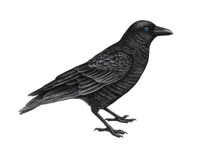
\includegraphics[width=3cm,height=2.5cm]{C5S01 – DT – Q1i.png}}},
  optionB={\adjustbox{scale=\scalefactor}{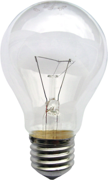
\includegraphics[width=1.5cm,height=2.5cm]{C5S01 – DT – Q1ii.png}}},
  optionC={\adjustbox{scale=\scalefactor}{
\includegraphics[width=3.5cm,height=2.5cm]{C5S01 – DT – Q1iii.png}}},
  optionD={\adjustbox{scale=\scalefactor}{
\includegraphics[width=2.5cm,height=2.5cm]{C5S01 – DT – Q1iv.png}}},
  correctoption={A},
}
% end-of-question
%-----------------------------------------------------------
%                        Question [  ]
%-----------------------------------------------------------
% start-of-question

\mcqtextbottomOneFour{
  questionnumber={2}, 
  questionTag={C5S01 – DT – Q2}, 
  questiontext={Which part of the plant absorbs water and nutrients from soil? },
  optionA={Flower},
  optionB={Stem},
  optionC={Leaves},
  optionD={Root},
  correctoption={D},
}

% end-of-question
%-----------------------------------------------------------
%                        Question [  ]
%-----------------------------------------------------------
% start-of-question

\mcqtextbottomOneFour{
  questionnumber={3}, 
  questionTag={C5S01 – DT – Q3}, 
  questiontext={Which of the following dog’s senses is very useful for humans?},
  optionA={Hearing},
  optionB={Smell},
  optionC={Taste},
  optionD={Touch},
  correctoption={B},
}

% end-of-question
%-----------------------------------------------------------
%                        Question [  ]
%-----------------------------------------------------------
% start-of-question
\mcqimgleftFourOne{
  questionnumber={4}, 
  questionTag={C5S01 – DT – Q4},
  questiontext={Match the following based on the parts for which the animals are hunted.},
  imgtabletikz= {\renewcommand{\arraystretch}{1.25}
\begin{tabular}{|p{0.25cm}|p{3cm}|p{0.25cm}|p{0.25cm}|p{3cm}|}
\hline
\multicolumn{2}{|c|}{Column A} & & \multicolumn{2}{|c|}{Column B} \\
\cline{1-2}\cline{4-5}
 i & Elephant & & a& Skin \\
\cline{1-2}\cline{4-5}
ii & Rhinoceros  & & b & Musk \\
\cline{1-2}\cline{4-5}
iii & Tiger and Snake & & c& Tusk \\
\cline{1-2}\cline{4-5}
iv & Musk deer & & d& Horn \\
\hline
\end{tabular}},
  optionA={i–d, ii–a, iii–b, iv–c },
  optionB={i–c, ii–b, iii–a, iv–d },
  optionC={i–b, ii–c, iii–a, iv–d },
  optionD={i–c, ii–d, iii–a, iv–b },
  correctoption={D},
  leftmini={0.5},
  rightmini={0.4},
}
% end-of-question
%-----------------------------------------------------------
%                        Question [  ]
%-----------------------------------------------------------
% start-of-question
\mcqtextbottomOneTwo{
  questionnumber={5}, 
  questionTag={C5S01 – DT – Q5}, 
  questiontext={Snakes have ears to protect them from enemies.},
  optionA={True},
  optionB={False},
   correctoption={B},
}
% end-of-question
%-----------------------------------------------------------
%                        Question [  ]
%-----------------------------------------------------------
% start-of-question
\mcqtextbottomOneTwo{
  questionnumber={6}, 
  questionTag={C5S01 – DT – Q6}, 
  questiontext={All types of snakes in India are poisonous.},
  optionA={True},
  optionB={False},
   correctoption={B},
}
% end-of-question
%-----------------------------------------------------------
%                        Question [ ]
%-----------------------------------------------------------
% start-of-question
\mcqtextbottomOneFour{
  questionnumber={1}, 
  questionTag={C5S02 – DT – Q1}, 
  questiontext={Find the healthiest food.},
  optionA={Fruits },
  optionB={French fries },
  optionC={Burger },
  optionD={Pizza },
  correctoption={A},
}
% end-of-question
%-----------------------------------------------------------
%                        Question [ ]
%-----------------------------------------------------------
% start-of-question
\mcqtextbottomOneFour{
  questionnumber={2}, 
  questionTag={C5S02 – DT – Q2}, 
  questiontext={The taste of an unripe mango is \rule{80pt}{0.5pt}.},
  optionA={Sour},
  optionB={Sweet},
  optionC={Bitter},
  optionD={Salt},
  correctoption={A},
}
% end-of-question
%-----------------------------------------------------------
%                        Question [ ]
%-----------------------------------------------------------
% start-of-question
\mcqtextbottomFourOne{
  questionnumber={3}, 
  questionTag={C5S02 – DT – Q3}, 
  questiontext={What is the purpose of the expiry date in packed food?},
  optionA={To identify the taste of the food using QR code.},
  optionB={To provide information on when the food was manufactured.},
  optionC={To ensure food is safe to eat.},
  optionD={To indicate the ingredients used in the food.},
  correctoption={C},
}
% end-of-question
%-----------------------------------------------------------
%                        Question [ ]
%-----------------------------------------------------------
% start-of-question
\mcqtextbottomFourOne{
  questionnumber={4}, 
  questionTag={C5S02 – DT – Q4}, 
  questiontext={What are all the factors needed to identify spoiled food?},
  optionA={Change in the colour and texture of the food},
  optionB={Unpleasant odour},
  optionC={Change in taste},
  optionD={All the above},
  correctoption={D},
}
% end-of-question
%-----------------------------------------------------------
%                        Question [ ]
%-----------------------------------------------------------
% start-of-question
\mcqtextbottomFourOne{
  questionnumber={5}, 
  questionTag={C5S02 – DT – Q5}, 
  questiontext={Why do living organisms need shelter?},
  optionA={To store water.},
  optionB={To prepare food.},
  optionC={To protect from extreme climate conditions.},
  optionD={To produce energy for survival.},
  correctoption={C},
}
% end-of-question

%-----------------------------------------------------------
%                        Question [ ]
%-----------------------------------------------------------
% start-of-question
\mcqtextbottomTwoTwo{
  questionnumber={1}, 
  questionTag={C5S03 – DT – Q1}, 
  questiontext={Find the incorrect pair based on parts of the human body and its function.},
  optionA={Tongue –  Taste},
  optionB={Ear - Chew},
  optionC={Nose - Smell},
  optionD={Eyes - Vision},
  correctoption={B},
}
% end-of-question
%-----------------------------------------------------------
%                        Question [  ]
%-----------------------------------------------------------
% start-of-question

\mcqtextbottomOneFour{
  questionnumber={2}, 
  questionTag={C5S03 – DT – Q2}, 
  questiontext={\rule{80pt}{0.5pt} helps doctor to hear the heartbeat of a person.},
  optionA={Stethoscope },
  optionB={Thermometer },
  optionC={Tablet },
  optionD={X ray},
  correctoption={A},
}

% end-of-question
%-----------------------------------------------------------
%                        Question [ ]
%-----------------------------------------------------------
% start-of-question
\mcqtextbottomFourOne{
  questionnumber={3}, 
  questionTag={C5S03 – DT – Q3}, 
  questiontext={Why should we eat the food slowly and chew them properly?},
  optionA={To identify the taste of the food.},
  optionB={It makes your teeth stronger.},
  optionC={This helps in the proper digestion of food.},
  optionD={To avoid eating too much of food.},
  correctoption={C},
}
% end-of-question
%-----------------------------------------------------------
%                        Question [ ]
%-----------------------------------------------------------
% start-of-question
\mcqtextbottomOneFour{
  questionnumber={4}, 
  questionTag={C5S03 – DT – Q4}, 
  questiontext={Which among the following diseases are not caused due to mosquitoes?},
  optionA={Malaria},
  optionB={Chikungunya},
  optionC={Chicken pox},
  optionD={Dengue},
  correctoption={C},
}
% end-of-question
%-----------------------------------------------------------
%                        Question [ ]
%-----------------------------------------------------------
% start-of-question
\mcqtextbottomOneFour{
  questionnumber={5}, 
  questionTag={C5S03 – DT – Q5}, 
  questiontext={Name the health condition of a person with less iron content in the blood.},
  optionA={Diarrhoea},
  optionB={Anaemia},
  optionC={Diabetes},
  optionD={Blood pressure},
  correctoption={B},
}
% end-of-question
%-----------------------------------------------------------
%                        Question [  ]
%-----------------------------------------------------------
% start-of-question
\mcqtextbottomOneTwo{
  questionnumber={6}, 
  questionTag={C5S03 – DT – Q6}, 
  questiontext={State True or False.\\Some diseases like cancer can be passed from parents to their children.},
  optionA={True},
  optionB={False},
   correctoption={A},
}
% end-of-question
%-----------------------------------------------------------
%                        Question [ ]
%-----------------------------------------------------------
% start-of-question
\mcqtextbottomTwoTwo{
  questionnumber={1}, 
  questionTag={C5S04 – DT – Q1}, 
  questiontext={Find the correct pair.},
  optionA={1 week – 6 days},
  optionB={1 year – 365 days},
  optionC={1 month – 25 days},
  optionD={1 decade – 1 year},
  correctoption={B},
}
% end-of-question
%-----------------------------------------------------------
%                        Question [ ]
%-----------------------------------------------------------
% start-of-question
\mcqtextbottomOneFour{
  questionnumber={2}, 
  questionTag={C5S04 – DT – Q2}, 
  questiontext={Identify the largest planet in solar system.},
  optionA={Earth},
  optionB={Mercury},
  optionC={Jupiter},
  optionD={Moon},
  correctoption={C},
}
% end-of-question%-----------------------------------------------------------
%                        Question [ ]
%-----------------------------------------------------------
% start-of-question
\mcqtextbottomOneFour{
  questionnumber={3}, 
  questionTag={C5S04 – DT – Q3}, 
  questiontext={Sun rises in the \rule{80pt}{0.5pt} and sets in the \rule{80pt}{0.5pt}.},
  optionA={South, North},
  optionB={North, South},
  optionC={West, East},
  optionD={East, West},
  correctoption={D},
}
% end-of-question%-----------------------------------------------------------
%                        Question [ ]
%-----------------------------------------------------------
% start-of-question
\mcqtextbottomOneFour{
  questionnumber={4}, 
  questionTag={C5S04 – DT – Q4}, 
  questiontext={The movement of the earth around the sun is called as \rule{80pt}{0.5pt}.},
  optionA={Orbit},
  optionB={Rotation},
  optionC={Revolution},
  optionD={Galaxy},
  correctoption={C},
}
% end-of-question%-----------------------------------------------------------
%                        Question [ ]
%-----------------------------------------------------------
% start-of-question
\mcqtextbottomFourOne{
  questionnumber={1}, 
  questionTag={C5S05 – DT – Q1}, 
  questiontext={What happens when you dry wet cloths under sun?},
  optionA={The colour of the cloths changes automatically into blue under sunlight.},
  optionB={The clothes become more wet due to sunlight.},
  optionC={The water disappears, leaving the clothes dry.},
  optionD={The size of the cloths becomes larger.},
  correctoption={C},
}
% end-of-question%-----------------------------------------------------------
%                        Question [ ]
%-----------------------------------------------------------
% start-of-question
\mcqtextbottomOneFour{
  questionnumber={2}, 
  questionTag={C5S05 – DT – Q2}, 
  questiontext={After the rain stops in the afternoon, what type of weather conditions would you experience?},
  optionA={Snow},
  optionB={Rain},
  optionC={Sunshine},
  optionD={Storm},
  correctoption={C},
}
% end-of-question%-----------------------------------------------------------
%                        Question [ ]
%-----------------------------------------------------------
% start-of-question
\mcqtextbottomOneFour{
  questionnumber={3}, 
  questionTag={C5S05 – DT – Q3}, 
  questiontext={Which among the following disasters brings a shake in the ground?},
  optionA={Flood },
  optionB={Earthquake },
  optionC={Lightning },
  optionD={Acid rain},
  correctoption={B},
}
% end-of-question%-----------------------------------------------------------
%                        Question [ ]
%-----------------------------------------------------------
% start-of-question
\mcqtextbottomOneFour{
  questionnumber={4}, 
  questionTag={C5S05 – DT – Q4}, 
  questiontext={Days are longer and nights and shorter in \rule{80pt}{0.5pt} season.},
  optionA={Winter},
  optionB={Spring},
  optionC={Summer},
  optionD={Autumn},
  correctoption={C},
}
% end-of-question%-----------------------------------------------------------
%                        Question [ ]
%-----------------------------------------------------------
% start-of-question
\mcqtextbottomFourOne{
  questionnumber={5}, 
  questionTag={C5S05 – DT – Q5}, 
  questiontext={Find the wrong measure taken during an earthquake.},
  optionA={Must leave the house and go to the open ground.},
  optionB={Seeking shelter under a strong piece of furniture.},
  optionC={Avoid elevators and use staircases for escape. },
  optionD={ Standing near windows for a better view.},
  correctoption={D},
}
% end-of-question%-----------------------------------------------------------
%                        Question [ ]
%-----------------------------------------------------------
% start-of-question
\mcqtextbottomOneFour{
  questionnumber={1}, 
  questionTag={C5S06 – DT – Q1}, 
  questiontext={In olden days, forest remained as a major source of \rule{80pt}{0.5pt} and \rule{80pt}{0.5pt} for humans. },
  optionA={Vacation, Running  },
  optionB={Trekking, Trading },
  optionC={Picnic, Medicine },
  optionD={Food, Medicine },
  correctoption={D},
}
% end-of-question
%-----------------------------------------------------------
%                        Question [  ]
%-----------------------------------------------------------
% start-of-question
\mcqtextbottomOneTwo{
  questionnumber={2}, 
  questionTag={C5S06 – DT – Q2}, 
  questiontext={State True or False.\\Some seeds can be moved from one place to another with the help of wind.},
  optionA={True},
  optionB={False},
   correctoption={A},
}
% end-of-question
%-----------------------------------------------------------
%                        Question [ ]
%-----------------------------------------------------------
% start-of-question
\mcqtextbottomOneFour{
  questionnumber={3}, 
  questionTag={C5S06 – DT – Q3}, 
  questiontext={Which among the following does not helps in seed dispersal?},
  optionA={Birds},
  optionB={Wind},
  optionC={Animals},
  optionD={Sunlight},
  correctoption={D},
}
% end-of-question%-----------------------------------------------------------
%                        Question [ ]
%-----------------------------------------------------------
% start-of-question
\mcqtextbottomTwoTwo{
  questionnumber={4}, 
  questionTag={C5S06 – DT – Q4}, 
  questiontext={What are the essential things needed for trekking?},
  optionA={Navigation tools like map and compass},
  optionB={First-aid kit},
  optionC={Food and Water},
  optionD={All of the above},
  correctoption={D},
}
% end-of-question%-----------------------------------------------------------
%                        Question [ ]
%-----------------------------------------------------------
% start-of-question
\mcqtextbottomOneFour{
  questionnumber={5}, 
  questionTag={C5S06 – DT – Q5}, 
  questiontext={Name the tallest mountain in the world.},
  optionA={Aanaimalai},
  optionB={Mount Everest},
  optionC={Aaravalli },
  optionD={Kanchenjunga},
  correctoption={B},
}
% end-of-question%-----------------------------------------------------------
%                        Question [ ]
%-----------------------------------------------------------
% start-of-question
\mcqtextbottomOneFour{
  questionnumber={6}, 
  questionTag={C5S06 – DT – Q6}, 
  questiontext={Find the incorrect one based on the use of fuel.},
  optionA={Car },
  optionB={Bike},
  optionC={Bicycle},
  optionD={Aeroplane},
  correctoption={C},
}
% end-of-question%-----------------------------------------------------------
%                        Question [ ]
%-----------------------------------------------------------
% start-of-question
\mcqtextbottomOneFour{
  questionnumber={7}, 
  questionTag={C5S06 – DT – Q7}, 
  questiontext={Which of the following is not a fuel?},
  optionA={Coal},
  optionB={Air},
  optionC={Diesel},
  optionD={Kerosene},
  correctoption={B},
}
% end-of-question%-----------------------------------------------------------
%                        Question [ ]
%-----------------------------------------------------------
% start-of-question
\mcqtextbottomOneFour{
  questionnumber={8}, 
  questionTag={C5S06 – DT – Q8}, 
  questiontext={Which of the following is not used as a fuel for cooking?},
  optionA={Wood},
  optionB={Dung cakes},
  optionC={Kerosene},
  optionD={Plastic bottle},
  correctoption={D},
}
% end-of-question%-----------------------------------------------------------
%                        Question [ ]
%-----------------------------------------------------------
% start-of-question
\mcqtextbottomOneFour{
  questionnumber={1}, 
  questionTag={C5S07 – DT – Q1}, 
  questiontext={Which among the following substance does not get attracted towards magnet?},
  optionA={Steel spoon },
  optionB={Iron rod},
  optionC={Eraser},
  optionD={Safety pin},
  correctoption={C},
}
% end-of-question%-----------------------------------------------------------
%                        Question [ ]
%-----------------------------------------------------------
% start-of-question
\mcqtextbottomOneFour{
  questionnumber={1}, 
  questionTag={C5S08 – DT – Q1}, 
  questiontext={Water turns into gas, when it is \rule{80pt}{0.5pt}.},
  optionA={Heated},
  optionB={Cooled},
  optionC={Left closed},
  optionD={Freezed},
  correctoption={A},
}
% end-of-question%-----------------------------------------------------------
%                        Question [ ]
%-----------------------------------------------------------
% start-of-question
\mcqtextbottomOneFour{
  questionnumber={2}, 
  questionTag={C5S08 – DT – Q2}, 
  questiontext={The water in the ocean is an example of \rule{80pt}{0.5pt} substance.},
  optionA={Liquid},
  optionB={Gas},
  optionC={Solid},
  optionD={Vacuum},
  correctoption={A},
}
% end-of-question
%-----------------------------------------------------------
%                        Question [ ]
%-----------------------------------------------------------
% start-of-question
\mcqtextbottomOneFour{
  questionnumber={3}, 
  questionTag={C5S08 – DT – Q3}, 
  questiontext={Rocks are tough to break because of its \rule{80pt}{0.5pt}.},
  optionA={Light weight },
  optionB={Hardness},
  optionC={Size},
  optionD={Shape},
  correctoption={B},
}
% end-of-question
%-----------------------------------------------------------
%                        Question [ ]
%-----------------------------------------------------------
% start-of-question
\mcqtextbottomOneFour{
  questionnumber={4}, 
  questionTag={C5S08 – DT – Q4}, 
  questiontext={Light can easily pass through glass material because of its \rule{80pt}{0.5pt}. },
  optionA={Transparency},
  optionB={Softness},
  optionC={Hardness},
  optionD={Light weight},
  correctoption={A},
}
% end-of-question
%-----------------------------------------------------------
%                        Question [ ]
%-----------------------------------------------------------
% start-of-question
\mcqtextbottomOneFour{
  questionnumber={1}, 
  questionTag={C5S09 – DT – Q1}, 
  questiontext={What type of energy is produced by burning candle?},
  optionA={Light},
  optionB={Sound},
  optionC={Heat},
  optionD={Both a and c},
  correctoption={D},
}
% end-of-question
%-----------------------------------------------------------
%                        Question [ ]
%-----------------------------------------------------------
% start-of-question
\mcqtextbottomFourOne{
  questionnumber={2}, 
  questionTag={C5S09 – DT – Q2}, 
  questiontext={Find the incorrect statement.},
  optionA={Hot food gets cooled down on blowing air over it.},
  optionB={Cold hand gets warmed up on blowing air.},
  optionC={Guitar produces music by blowing air on its strings. },
  optionD={Paper whistle produces sound on blowing air into it.},
  correctoption={C},
}
% end-of-question
%-----------------------------------------------------------
%                        Question [ ]
%-----------------------------------------------------------
% start-of-question
\mcqtextbottomOneFour{
  questionnumber={3}, 
  questionTag={C5S09 – DT – Q3}, 
  questiontext={What is the main natural source of light for the living beings on earth?},
  optionA={Moon},
  optionB={Star},
  optionC={Sun},
  optionD={Fire},
  correctoption={C},
}
% end-of-question
%-----------------------------------------------------------
%                        Question [ ]
%-----------------------------------------------------------
% start-of-question
\mcqtextbottomFourOne{
  questionnumber={1}, 
  questionTag={C5S10 – DT – Q1}, 
  questiontext={What is the first aid for a minor burn in your hand?},
  optionA={Apply oil as an ointment over the burn area.},
  optionB={Rinse the burn area with cool water.},
  optionC={Apply salt over the burn area.},
  optionD={Cover the burn with plastic paper immediately.},
  correctoption={B},
}
% end-of-question
%-----------------------------------------------------------
%                        Question [ ]
%-----------------------------------------------------------
% start-of-question
\mcqtextbottomOneFour{
  questionnumber={2}, 
  questionTag={C5S10 – DT – Q2}, 
  questiontext={What is the medical emergency number in India?},
  optionA={108},
  optionB={100},
  optionC={101},
  optionD={911},
  correctoption={A},
}
% end-of-question
%-----------------------------------------------------------
%                        Question [ ]
%-----------------------------------------------------------
% start-of-question
\mcqtextbottomFourOne{
  questionnumber={3}, 
  questionTag={C5S10 – DT – Q3}, 
  questiontext={Which of the following is not a safety precaution when crossing the road?},
  optionA={Running across the road when cars are passing by.},
  optionB={Follow proper traffic signals and signs.},
  optionC={Looking left and right before crossing the road.},
  optionD={Cross roads where there is signal of crosswalks.},
  correctoption={A},
}
% end-of-question

%-----------------------------------------------------------
%                        Question [ 215 ]
%-----------------------------------------------------------
% start-of-question

\mcqtextbottomOneFour{
  questionnumber={1}, 
  questionTag={C5S09 – DT – Q4}, 
  questiontext={Identify which of the following non-living beings can produce light.},
  optionA={
  \adjustbox{scale=\scalefactor}{
\tikzset{every picture/.style={line width=0.75pt}} 
\begin{tikzpicture}[x=0.75pt,y=0.75pt,yscale=-1,xscale=1]
\draw (91.5,99.3) node  {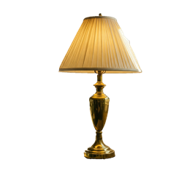
\includegraphics[width=86.25pt,height=72.45pt]{C5PS – DT – Q1i.png}};
\draw (46,150.2) node [anchor=north west][inner sep=0.75pt]   [align=left] {Lamp};
\end{tikzpicture} }
},
optionB={\adjustbox{scale=\scalefactor}{
\tikzset{every picture/.style={line width=0.75pt}} 
\begin{tikzpicture}[x=0.75pt,y=0.75pt,yscale=-1,xscale=1]
\draw (84.5,96.3) node  {
\includegraphics[width=58.75pt,height=75.45pt]{C5PS – DT – Q1ii.png}};
\draw (39,152) node [anchor=north west][inner sep=0.75pt]   [align=left] {Lighting bees};
\end{tikzpicture}}
},
optionC={\adjustbox{scale=\scalefactor}{
\tikzset{every picture/.style={line width=0.75pt}}     
\begin{tikzpicture}[x=0.75pt,y=0.75pt,yscale=-1,xscale=1]
\draw (87.2,160.3) node  {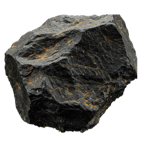
\includegraphics[width=79pt,height=73.95pt]{C5PS – DT – Q1iii.png}};
\draw (42,213) node [anchor=north west][inner sep=0.75pt]   [align=left] {Rock};
\end{tikzpicture}}
},
optionD={\adjustbox{scale=\scalefactor}{
\tikzset{every picture/.style={line width=0.75pt}} 
\begin{tikzpicture}[x=0.75pt,y=0.75pt,yscale=-1,xscale=1]
\draw (78.2,108.8) node  {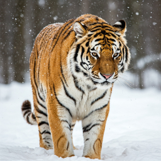
\includegraphics[width=84.9pt,height=74.7pt]{C5PS – DT – Q1iv.png}};
\draw (34,162) node [anchor=north west][inner sep=0.75pt]   [align=left] {Tiger};
\end{tikzpicture}}
},
correctoption={A},
}

% end-of-question

%-----------------------------------------------------------
%                        Question [ ]
%-----------------------------------------------------------
% start-of-question
\mcqtextbottomOneFour{
  questionnumber={2}, 
  questionTag={C5S09 – DT – Q5}, 
  questiontext={An apple falls from a tree to the ground due to \rule{80pt}{0.5pt}},
  optionA={Magnetic energy},
  optionB={Gravity},
  optionC={Light energy},
  optionD={Electricity},
  correctoption={B},
}
% end-of-question

%-----------------------------------------------------------
%                        Question [ ]
%-----------------------------------------------------------
% start-of-question
\mcqtextbottomOneFour{
  questionnumber={6}, 
  questionTag={C5S08 – DT – Q5}, 
  questiontext={Which of the following materials will sink in water?},
  optionA={Stone},
  optionB={Wooden stick},
  optionC={Dry leaf},
  optionD={Plastic bottle},
  correctoption={A},
}
% end-of-question
%-----------------------------------------------------------
%                        Question [ ]
%-----------------------------------------------------------
% start-of-question
\mcqtextbottomOneFour{
  questionnumber={4}, 
  questionTag={C5S08 – DT – Q6}, 
  questiontext={Which of the following materials allows you to see objects clearly on the other side?},
  optionA={Glass door},
  optionB={Wooden door},
  optionC={Metal door},
  optionD={All the above},
  correctoption={A},
}
% end-of-question

%-----------------------------------------------------------
%                        Question [ ]
%-----------------------------------------------------------
% start-of-question
\mcqtextbottomTwoTwo{
  questionnumber={5}, 
  questionTag={C5S02 – DT – Q6}, 
  questiontext={Why do we separate stones from rice before cooking? },
  optionA={To make food taste better.},
  optionB={To change the color of rice},
  optionC={To play with the picked stone from the rice},
  optionD={To remove harmful or unwanted materials },
  correctoption={D},
}
% end-of-question

%-----------------------------------------------------------
%                        Question [ ]
%-----------------------------------------------------------
% start-of-question
\mcqtextbottomOneFour{
  questionnumber={6}, 
  questionTag={C5S09 – DT – Q6}, 
  questiontext={Which of the following feels hot when touched?},
  optionA={Burning candle},
  optionB={Ice cube},
  optionC={Plastic toy},
  optionD={Cotton cloth},
  correctoption={A},
}
% end-of-question

%-----------------------------------------------------------
%                        Question [ ]
%-----------------------------------------------------------
% start-of-question
\mcqtextbottomTwoTwo{
  questionnumber={1}, 
  questionTag={C5S02 – DT – Q7}, 
  questiontext={Why do we feel tired if we skip breakfast?},
  optionA={Our stomach gets too full.},
  optionB={Our body lacks energy.},
  optionC={Feel sleepy because of no rest},
  optionD={Due to the over-workout},
  correctoption={B},
}
% end-of-question
%-----------------------------------------------------------
%                        Question [ ]
%-----------------------------------------------------------
% start-of-question
\mcqtextbottomOneFour{
  questionnumber={2}, 
  questionTag={C5S02 – DT – Q8}, 
  questiontext={Which of these comes from a cow?},
  optionA={Wool},
  optionB={Milk},
  optionC={Eggs},
  optionD={Silk},
  correctoption={B},
}
% end-of-question

%-----------------------------------------------------------
%                        Question [ 1 ]
%-----------------------------------------------------------
% start-of-question
\mcqtextbottomOneFour{
  questionnumber={3}, 
  questionTag={C5S01 – DT – Q7}, 
  questiontext={Which of these animals can live both in water and on land?},
  optionA={\adjustbox{scale=\scalefactor}{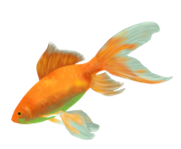
\includegraphics[width=3cm,height=2.5cm]{C5BZ – DT – Q3i.png}}},
  optionB={\adjustbox{scale=\scalefactor}{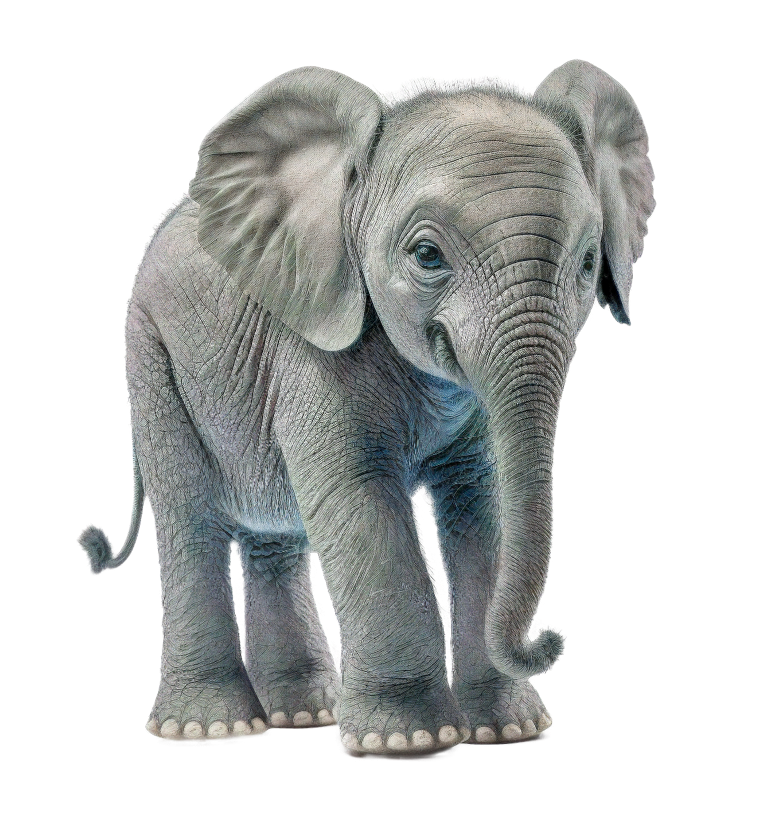
\includegraphics[width=3cm,height=2.5cm]{C5BZ – DT – Q3ii.png}}},
  optionC={\adjustbox{scale=\scalefactor}{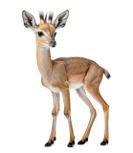
\includegraphics[width=3cm,height=2.5cm]{C5BZ – DT – Q3iii.png}}},
  optionD={\adjustbox{scale=\scalefactor}{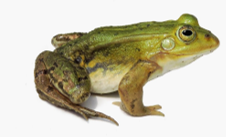
\includegraphics[width=3cm,height=2.5cm]{C5BZ – DT – Q3iv.png}}},
  correctoption={D},
}
% end-of-question

%-----------------------------------------------------------
%                        Question [ ]
%-----------------------------------------------------------
% start-of-question
\mcqtextbottomOneFour{
  questionnumber={4}, 
  questionTag={C5S01 – DT – Q8}, 
  questiontext={Which body part helps a bird to fly?},
  optionA={Legs},
  optionB={Eyes},
  optionC={Wings},
  optionD={Tail},
  correctoption={C},
}
% end-of-question
%-----------------------------------------------------------
%                        Question [ ]
%-----------------------------------------------------------
% start-of-question
\mcqtextbottomTwoTwo{
  questionnumber={1}, 
  questionTag={C5S02 – DT – Q9}, 
  questiontext={What should we do to save water?},
  optionA={Leave the tap running while washing dishes.},
  optionB={Watering the plants during rain.},
  optionC={Take long showers every day.},
  optionD={Turn off the taps when not in use},
  correctoption={D},
}
% end-of-question

%-----------------------------------------------------------
%                        Question [ ]
%-----------------------------------------------------------
% start-of-question
\mcqtextbottomTwoTwo{
  questionnumber={2}, 
  questionTag={C5S06 – DT – Q9}, 
  questiontext={Which of the following activity cause pollution?},
  optionA={Planting trees in a garden},
  optionB={Drinking clean water},
  optionC={Throwing plastic products into the river},
  optionD={Using cloth bags for shopping},
  correctoption={C},
}
% end-of-question

%-----------------------------------------------------------
%                        Question [ ]
%-----------------------------------------------------------
% start-of-question
\mcqtextbottomOneFour{
  questionnumber={3}, 
  questionTag={C5S02 – DT – Q10}, 
  questiontext={Which of these is a natural source of water?},
  optionA={Rain water},
  optionB={Purified water},
  optionC={Tap water},
  optionD={Boiled water},
  correctoption={A},
}
% end-of-question
%-----------------------------------------------------------
%                        Question [ ]
%-----------------------------------------------------------
% start-of-question
\mcqtextbottomTwoTwo{
  questionnumber={4}, 
  questionTag={C5S02 – DT – Q11}, 
  questiontext={Where can we find air?},
  optionA={Only in trees},
  optionB={Only in sky},
  optionC={Everywhere around us},
  optionD={Only in water},
  correctoption={C},
}
% end-of-question

\end{document}